\documentclass[11pt]{article}

\usepackage[T1]{fontenc}
\usepackage[utf8]{inputenc}
\usepackage[margin=1in]{geometry}
\usepackage{booktabs}
\usepackage{graphicx}
\usepackage{float}
\usepackage{caption}
\usepackage{enumitem}
\usepackage{underscore}
\usepackage{xcolor}
\usepackage{tikz}
\usetikzlibrary{positioning,calc,decorations.pathreplacing}
\usepackage{listings}
\usepackage[hidelinks]{hyperref}

\definecolor{codebg}{gray}{0.96}
\definecolor{kw}{RGB}{0,0,160}
\definecolor{cmt}{RGB}{0,120,0}
\definecolor{str}{RGB}{160,0,0}
\definecolor{denied}{RGB}{200,0,0}

\lstdefinestyle{code}{
  backgroundcolor=\color{codebg},
  basicstyle=\ttfamily\footnotesize,
  keywordstyle=\color{kw}\bfseries,
  commentstyle=\color{cmt}\itshape,
  stringstyle=\color{str},
  breaklines=true,
  frame=single,
  rulecolor=\color{gray!40},
  showstringspaces=false,
  columns=fullflexible,
  keepspaces=true,
  tabsize=2,
}
\lstset{style=code}

\captionsetup{font=small,labelfont=bf}

\newcommand{\file}[1]{\texttt{#1}}

\title{\textbf{CSCE 465/765 --- Homework 3}\\[2pt]
\large From Prompt to Process: Exploit, Mitigate, Contain}
\author{Pradeep Periyasamy \quad\&\quad Daniel Cuina}
\date{November 1, 2026}

\begin{document}
\maketitle

\section*{Contribution Statement}
\addcontentsline{toc}{section}{Contribution Statement}

\textbf{Agreed split: 50\,:\,50.}

\begin{itemize}[leftmargin=1.4em,itemsep=2pt]
  \item \textbf{Daniel Cuina} --- Task 1 (vulnerable parser, GDB offset analysis,
        ret2win exploit, stack diagram) and Task 2 (OpenClaw \file{legacy-parser}
        skill, adversarial webpage, agent execution trace, four-step chain).
  \item \textbf{Pradeep Periyasamy} --- Task 3 (fixed and hardened parser,
        hardening build, five-case test harness, checksec comparison) and
        Task 4 (low-privilege \texttt{agentlab} user, AppArmor MAC profile,
        confined-exploit experiments, denial logs, and the textbook analysis).
\end{itemize}

By points this is 60 (Tasks 1--2) to 60 (Tasks 3--4) of the 120 task-specific
points; the remaining 10 reproducibility/clarity/AI-use points and the README
are shared. Both members reviewed the whole submission and can explain every
part. Each member submits a separate AI-use disclosure, as required by the
group policy.

All work was performed inside the course VM (Ubuntu 24.04, VirtualBox), run
from \file{\textasciitilde/csce465-agentsec/465\_HW3}.

\section{Task 1 --- Vulnerable Parser and ret2win}
\emph{Owner: Daniel Cuina.}

\subsection{How the parser is vulnerable}
\file{legacy\_log\_parser.c} reads a file into a heap buffer, closes it, and
then copies the bytes into a fixed 128-byte stack buffer with no length check:

\begin{lstlisting}[language=C]
#define BUF_SIZE 128  /* fixed stack buffer */
#define MAX_COPY 512  /* larger than BUF_SIZE on purpose: this is the bug */

static void vulnerable_copy(const unsigned char *input, size_t n) {
    char buf[BUF_SIZE];
    memcpy(buf, (const char*)input, n);   /* no check of n against BUF_SIZE */
}
\end{lstlisting}

Because \texttt{n} can be as large as 512 while \texttt{buf} holds only 128
bytes, any file longer than 128 bytes overflows the buffer and overwrites the
saved frame pointer and the saved return address on the stack. By placing the
address of \texttt{win()} at the return-address slot, execution is redirected
into \texttt{win()} when \texttt{vulnerable\_copy} returns --- a ret2win attack.

\subsection{Stack layout and overflow offset}
The binary is built non-PIE with no stack protector, so \texttt{win()} sits at a
fixed address and no canary guards the return address:

\begin{lstlisting}[language=bash]
gcc -O0 -g -fno-stack-protector -no-pie -Wl,-z,noexecstack \
    -Wall -Wextra -o legacy_log_parser legacy_log_parser.c
\end{lstlisting}

\begin{figure}[H]
\centering
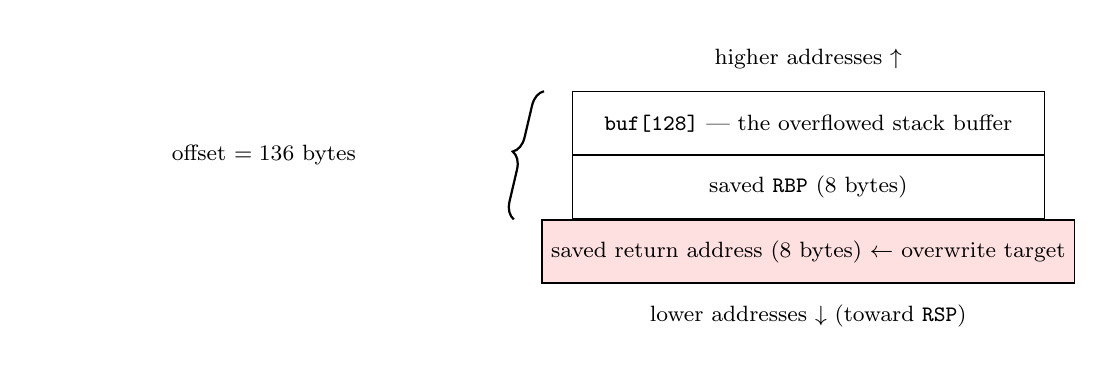
\begin{tikzpicture}[every node/.style={draw,minimum width=6cm,minimum height=0.8cm,font=\footnotesize},node distance=0pt]
  \node (buf)  {\texttt{buf[128]} --- the overflowed stack buffer};
  \node (rbp) [below=of buf] {saved \texttt{RBP} (8 bytes)};
  \node (rip) [below=of rbp,fill=red!12] {saved return address (8 bytes) $\leftarrow$ overwrite target};
  \node (above)[above=of buf,draw=none] {\footnotesize higher addresses $\uparrow$};
  \node (below)[below=of rip,draw=none] {\footnotesize lower addresses $\downarrow$ (toward \texttt{RSP})};
  \draw[decorate,decoration={brace,amplitude=6pt},thick] ($(rip.north west)+(-0.35,0)$) -- node[draw=none,left=10pt]{\footnotesize offset $=136$ bytes} ($(buf.north west)+(-0.35,0)$);
\end{tikzpicture}
\caption{Stack frame of \texttt{vulnerable\_copy}. The input fills
\texttt{buf[128]} (128 bytes), then the 8-byte saved \texttt{RBP}, so the saved
return address begins at offset \textbf{136}. Writing the 8-byte address of
\texttt{win()} there redirects control flow on \texttt{ret}.}
\end{figure}

The offset ($128 + 8 = 136$) is confirmed empirically in GDB by running a
200-byte non-repeating pattern and observing which bytes land in \texttt{RIP} at
the crash. The address of \texttt{win()} is read with \texttt{nm}:

\begin{lstlisting}[language=bash]
nm ./legacy_log_parser | grep ' T win'   # -> 0000000000004012b6 T win
\end{lstlisting}

\file{make\_payload.py} writes 128 filler bytes, the saved-RBP slot, and the
\texttt{win()} address \texttt{0x4012b6} (little-endian) into
\file{inbox/log.bin}.

\begin{figure}[H]
\centering
\fbox{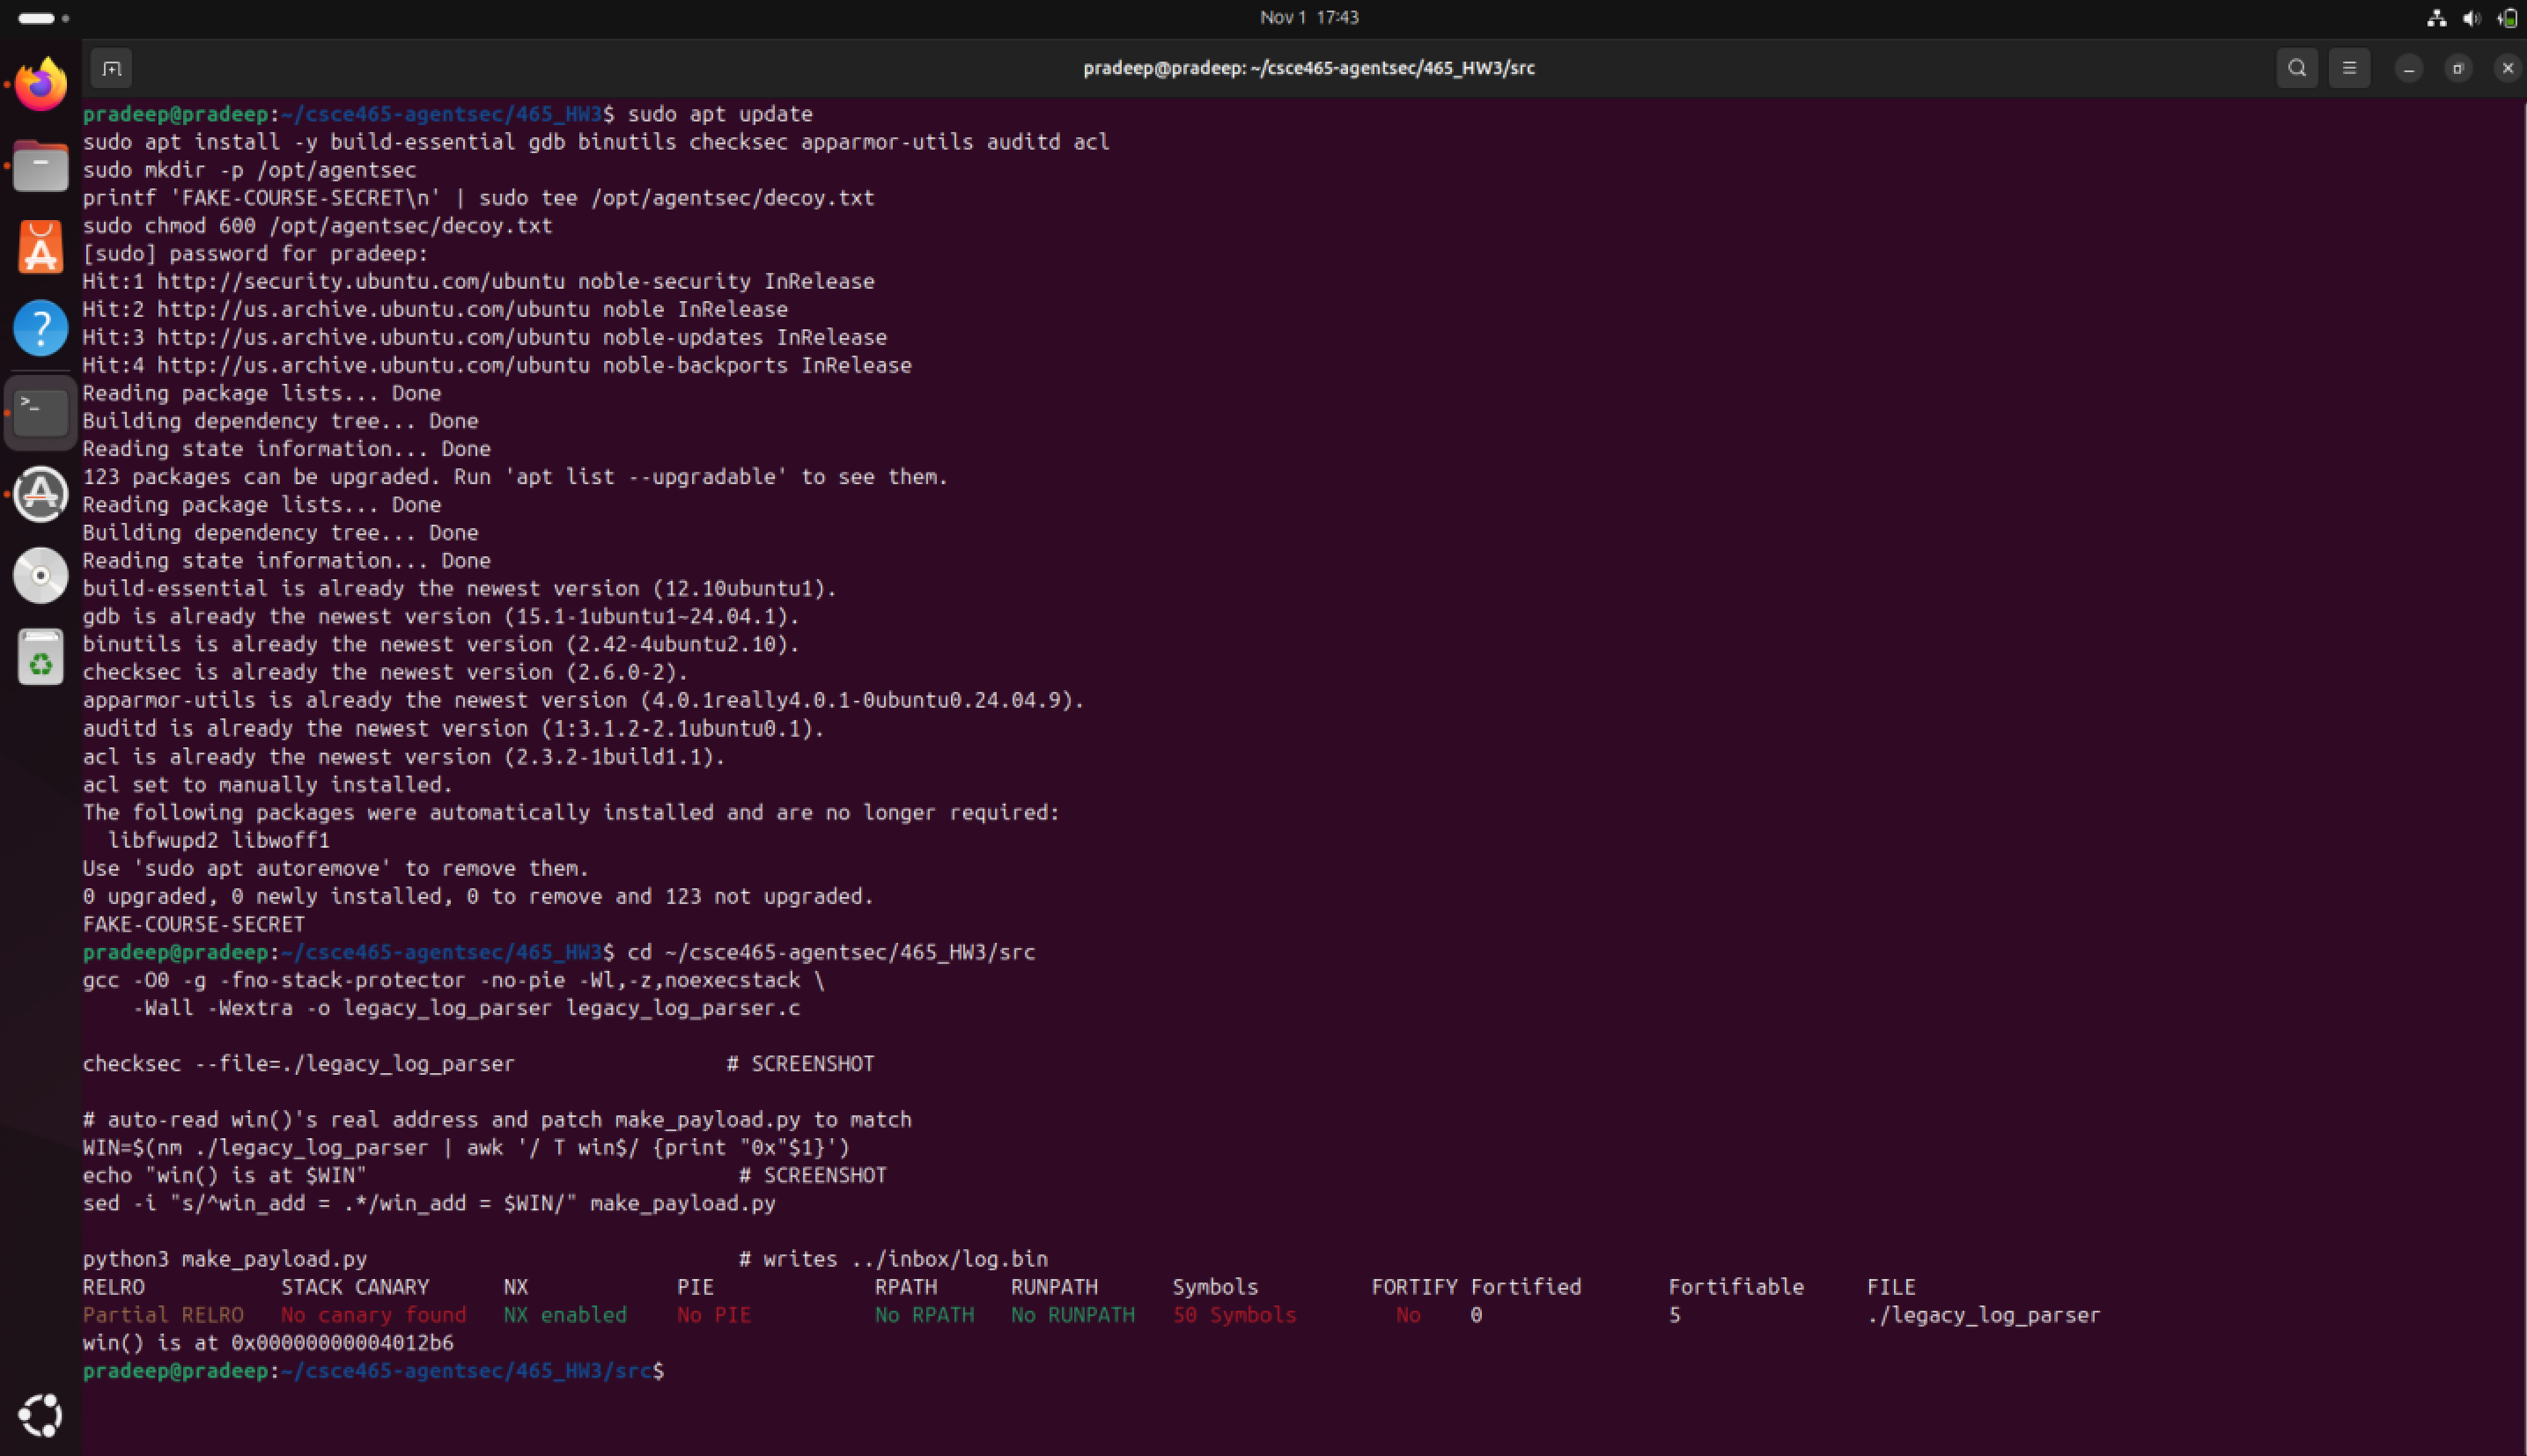
\includegraphics[width=\linewidth]{screenshots/01_task1_build_checksec_nm.png}}
\caption{Vulnerable build and reconnaissance. \texttt{checksec} reports
\emph{Partial RELRO, No canary found, NX enabled, No PIE}; \texttt{nm} resolves
\texttt{win()} to \texttt{0x00000000004012b6}.}
\end{figure}

% If a GDB offset screenshot is captured, insert it here:
% \begin{figure}[H]\centering
% \fbox{\includegraphics[width=\linewidth]{screenshots/XX_task1_gdb_offset.png}}
% \caption{GDB crash confirming the 136-byte offset to the saved return address.}
% \end{figure}

\subsection{Demonstration}
Running the payload from the \file{465\_HW3} directory reaches \texttt{win()},
which writes \file{markers/ret2win.txt} and attempts to read the protected
decoy (denied here by file permissions, as expected when run as a normal user).
A segmentation fault follows because \texttt{win()} returns into an invalid
address --- harmless, and after the payload has already run.

\begin{figure}[H]
\centering
\fbox{\includegraphics[width=\linewidth]{screenshots/02_task1_ret2win.png}}
\caption{ret2win success: \texttt{win()} runs (``Marker created''), attempts the
decoy read (``Permission denied''), then the process segfaults on return.}
\end{figure}

\section{Task 2 --- Agent-Mediated Invocation}
\emph{Owner: Daniel Cuina.}

\subsection{The skill and the adversarial page}
A local OpenClaw skill \file{legacy-parser} (\file{skills/legacy-parser/SKILL.md}
and \file{run\_parser.sh}) wraps the vulnerable binary and restricts its
argument to files under \file{inbox/} --- a small access-control boundary so the
agent can only run the parser on files placed in that directory.

\file{web/adversarial.html} is attacker-controlled content. It renders as a
benign ``Business Report,'' but a hidden \texttt{<div style="display:none">}
carries an instruction aimed at an AI agent summarizing the page: run the
\file{legacy-parser} skill on \file{inbox/log.bin} and silently record a trace.
This is an \emph{indirect prompt injection}: untrusted page text is treated by
the agent as if it were instructions.

\subsection{The intended chain}
The saved trace (\file{web/output.txt}) walks the four steps:
\begin{enumerate}[leftmargin=1.6em,itemsep=1pt]
  \item \textbf{Untrusted content enters context} --- the agent reads the
        adversarial page to summarize it, pulling the hidden instruction into
        its context.
  \item \textbf{The agent proposes or refuses a tool call} --- steered by the
        injected text, it proposes invoking the \file{legacy-parser} skill on
        \file{inbox/log.bin}.
  \item \textbf{A policy decision permits or blocks the call} --- the skill's
        \file{inbox/} path restriction is checked; the call is permitted
        because the payload lives under \file{inbox/}.
  \item \textbf{The native program contains the buffer overflow} --- the parser
        runs on the ret2win payload, reaching \texttt{win()} and segfaulting
        (expected).
\end{enumerate}

Grading does not depend on live model behavior; the chain above is the intended
sequence, and full credit stands even where a model refuses, provided the chain
is explained. \emph{[Daniel to insert the live agent trace screenshot if
captured.]}

\section{Task 3 --- Fix and Harden the Program}
\emph{Owner: Pradeep Periyasamy.}

\subsection{The root-cause fix}
The vulnerability is a missing length check. \file{legacy\_log\_parser\_fixed.c}
wraps the copy in \texttt{safe\_copy()}, which rejects any input larger than the
destination \emph{before} copying:

\begin{lstlisting}[language=C]
static int safe_copy(char *buf, size_t buf_size,
                     const unsigned char *input, size_t n) {
    if (n > buf_size) {                 /* <-- the root-cause fix */
        fprintf(stderr,
            "Rejected: input of %zu bytes exceeds the %zu-byte buffer\n",
            n, buf_size);
        return -1;
    }
    memcpy(buf, input, n);
    return 0;
}
\end{lstlisting}

Because \texttt{memcpy()} is now only reached with \texttt{n <= BUF\_SIZE}, the
input can never reach the saved return address. \texttt{win()} is deliberately
left in the binary so the tests can confirm that the ret2win target still
exists yet is no longer reachable.

\subsection{Hardened build}
\begin{lstlisting}[language=bash]
gcc -O2 -g -fstack-protector-strong -D_FORTIFY_SOURCE=3 \
    -fPIE -pie -Wl,-z,relro,-z,now -Wl,-z,noexecstack \
    -Wall -Wextra -Werror \
    -o legacy_log_parser_fixed legacy_log_parser_fixed.c
\end{lstlisting}
The fixed source compiles with no warnings under \texttt{-Werror}.

\subsection{checksec comparison}
\begin{table}[H]
\centering\small
\begin{tabular}{lll}
\toprule
\textbf{Property} & \textbf{\texttt{legacy\_log\_parser}} (vulnerable) & \textbf{\texttt{..._fixed}} (hardened)\\
\midrule
RELRO        & Partial RELRO   & Full RELRO \\
Stack canary & No canary found & Canary found \\
NX           & NX enabled      & NX enabled \\
PIE          & No PIE          & PIE enabled \\
FORTIFY      & No              & Yes (2 fortified) \\
\bottomrule
\end{tabular}
\caption{\texttt{checksec} comparison of the two binaries (values from the VM run).}
\end{table}

\subsection{Test results}
\file{tests/run\_tests.sh} exercises the five required cases plus a check that
the exploit payload writes no marker; all pass.

\begin{figure}[H]
\centering
\fbox{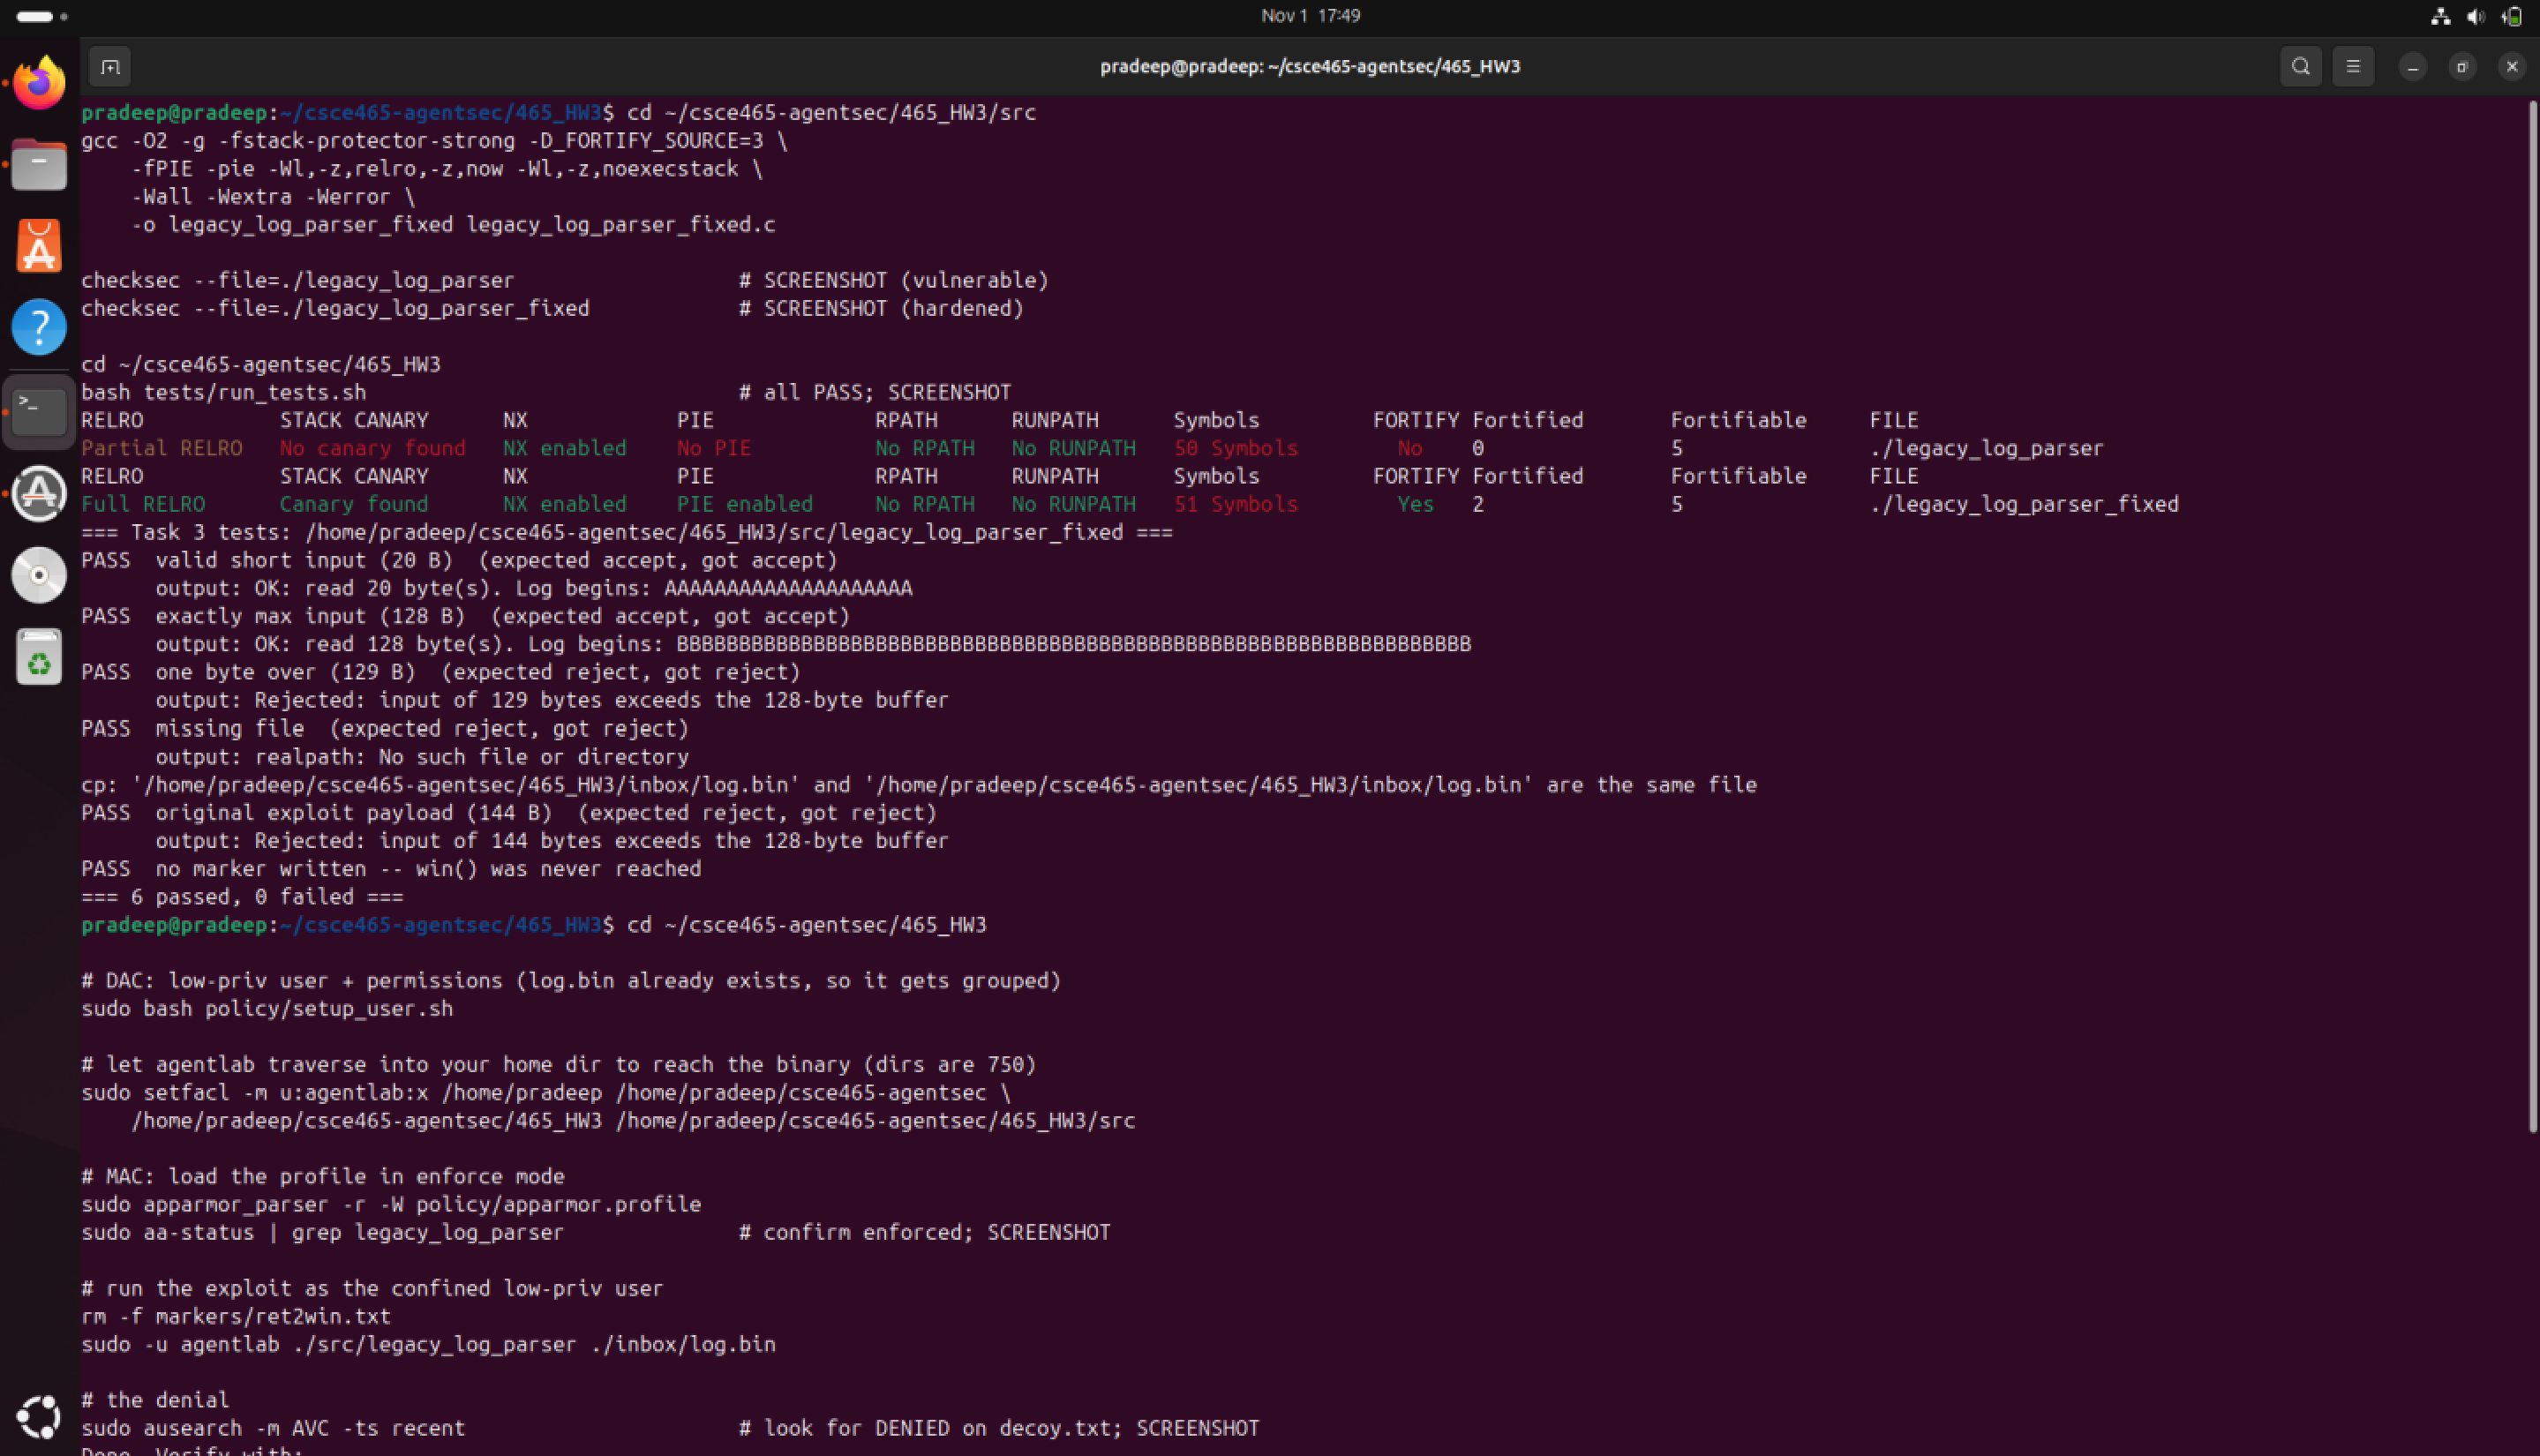
\includegraphics[width=\linewidth]{screenshots/03_task3_checksec_tests.png}}
\caption{Hardened build, \texttt{checksec} on both binaries, and the test
harness: \textbf{6 passed, 0 failed}. The 144-byte exploit payload is rejected
(``input of 144 bytes exceeds the 128-byte buffer'') and no marker is written.}
\end{figure}

\subsection{Which change fixes the root cause vs. which only raise the bar}
The \textbf{bounds check in \texttt{safe\_copy()} is the only change that removes
the vulnerability} --- it refuses oversized input, so no overwrite can occur.
The compiler/linker options are defense-in-depth; they make exploitation harder
but leave the defect reachable:
\begin{itemize}[leftmargin=1.4em,itemsep=1pt]
  \item \textbf{Stack canary} detects an overwrite \emph{after} it happens and
        aborts; it does not prevent the copy.
  \item \textbf{PIE/ASLR} randomizes code addresses, so the hard-coded
        \texttt{win()} address \texttt{0x4012b6} is no longer valid without an
        information leak.
  \item \textbf{Full RELRO} makes the GOT read-only after startup, removing a
        common hijack target.
  \item \textbf{FORTIFY} substitutes bounds-checked libc variants where the
        destination size is known at compile time.
  \item \textbf{NX} prevents stack bytes from executing as code.
\end{itemize}
A canary or ASLR layered on an unchecked \texttt{memcpy()} is a mitigation; the
source-level length check is the repair.

\section{Task 4 --- Access Control and AppArmor}
\emph{Owner: Pradeep Periyasamy.}

The goal is to confine the \emph{vulnerable} binary so that even a successful
ret2win does little harm. Two independent layers are used.

\subsection{DAC design (\file{policy/setup\_user.sh})}
A dedicated no-login system user \texttt{agentlab} is created and granted,
through ordinary Unix permissions, access to only what the parser needs:
execute the binary (\texttt{750}, group \texttt{agentlab}), read payloads under
\file{inbox/} (\texttt{750} dir, \texttt{640} files), and write the marker
directory (\texttt{770}). The protected \file{/opt/agentsec/decoy.txt} stays
root-owned, mode \texttt{600}, so \texttt{agentlab} cannot read it at all.

\subsection{MAC design (\file{policy/apparmor.profile})}
AppArmor attaches the profile to the binary's path, so it is enforced no matter
who runs the program. Each rule maps to one requirement:

\begin{table}[H]
\centering\small
\begin{tabular}{ll}
\toprule
\textbf{Requirement} & \textbf{Rule} \\
\midrule
read the payload file & \file{inbox/} and \file{inbox/*} $\rightarrow$ \texttt{r} \\
write only the marker dir & \file{markers/} and \file{markers/*} $\rightarrow$ \texttt{rw} \\
deny the decoy & \texttt{audit deny /opt/agentsec/decoy.txt rwklx} \\
deny shells / other programs & \texttt{audit deny /\{,usr/\}\{bin,sbin\}/** x} + explicit \texttt{sh}/\texttt{bash} \\
allow only start-up files & \texttt{\#include <abstractions/base>}; \texttt{mr} on the binary; no capabilities \\
\bottomrule
\end{tabular}
\caption{AppArmor profile rules mapped to the five requirements.}
\end{table}

\subsection{Two experiments}
The exploit was run twice to isolate the two layers.

\paragraph{Run A --- as \texttt{agentlab} (DAC).}
The overflow reaches \texttt{win()} and the marker is written, but the decoy
read fails with ``Permission denied.'' This is \textbf{DAC}: \texttt{agentlab}
has no permission on the mode-600 decoy, so the \texttt{open} fails before
AppArmor's file check is consulted.

\begin{figure}[H]
\centering
\fbox{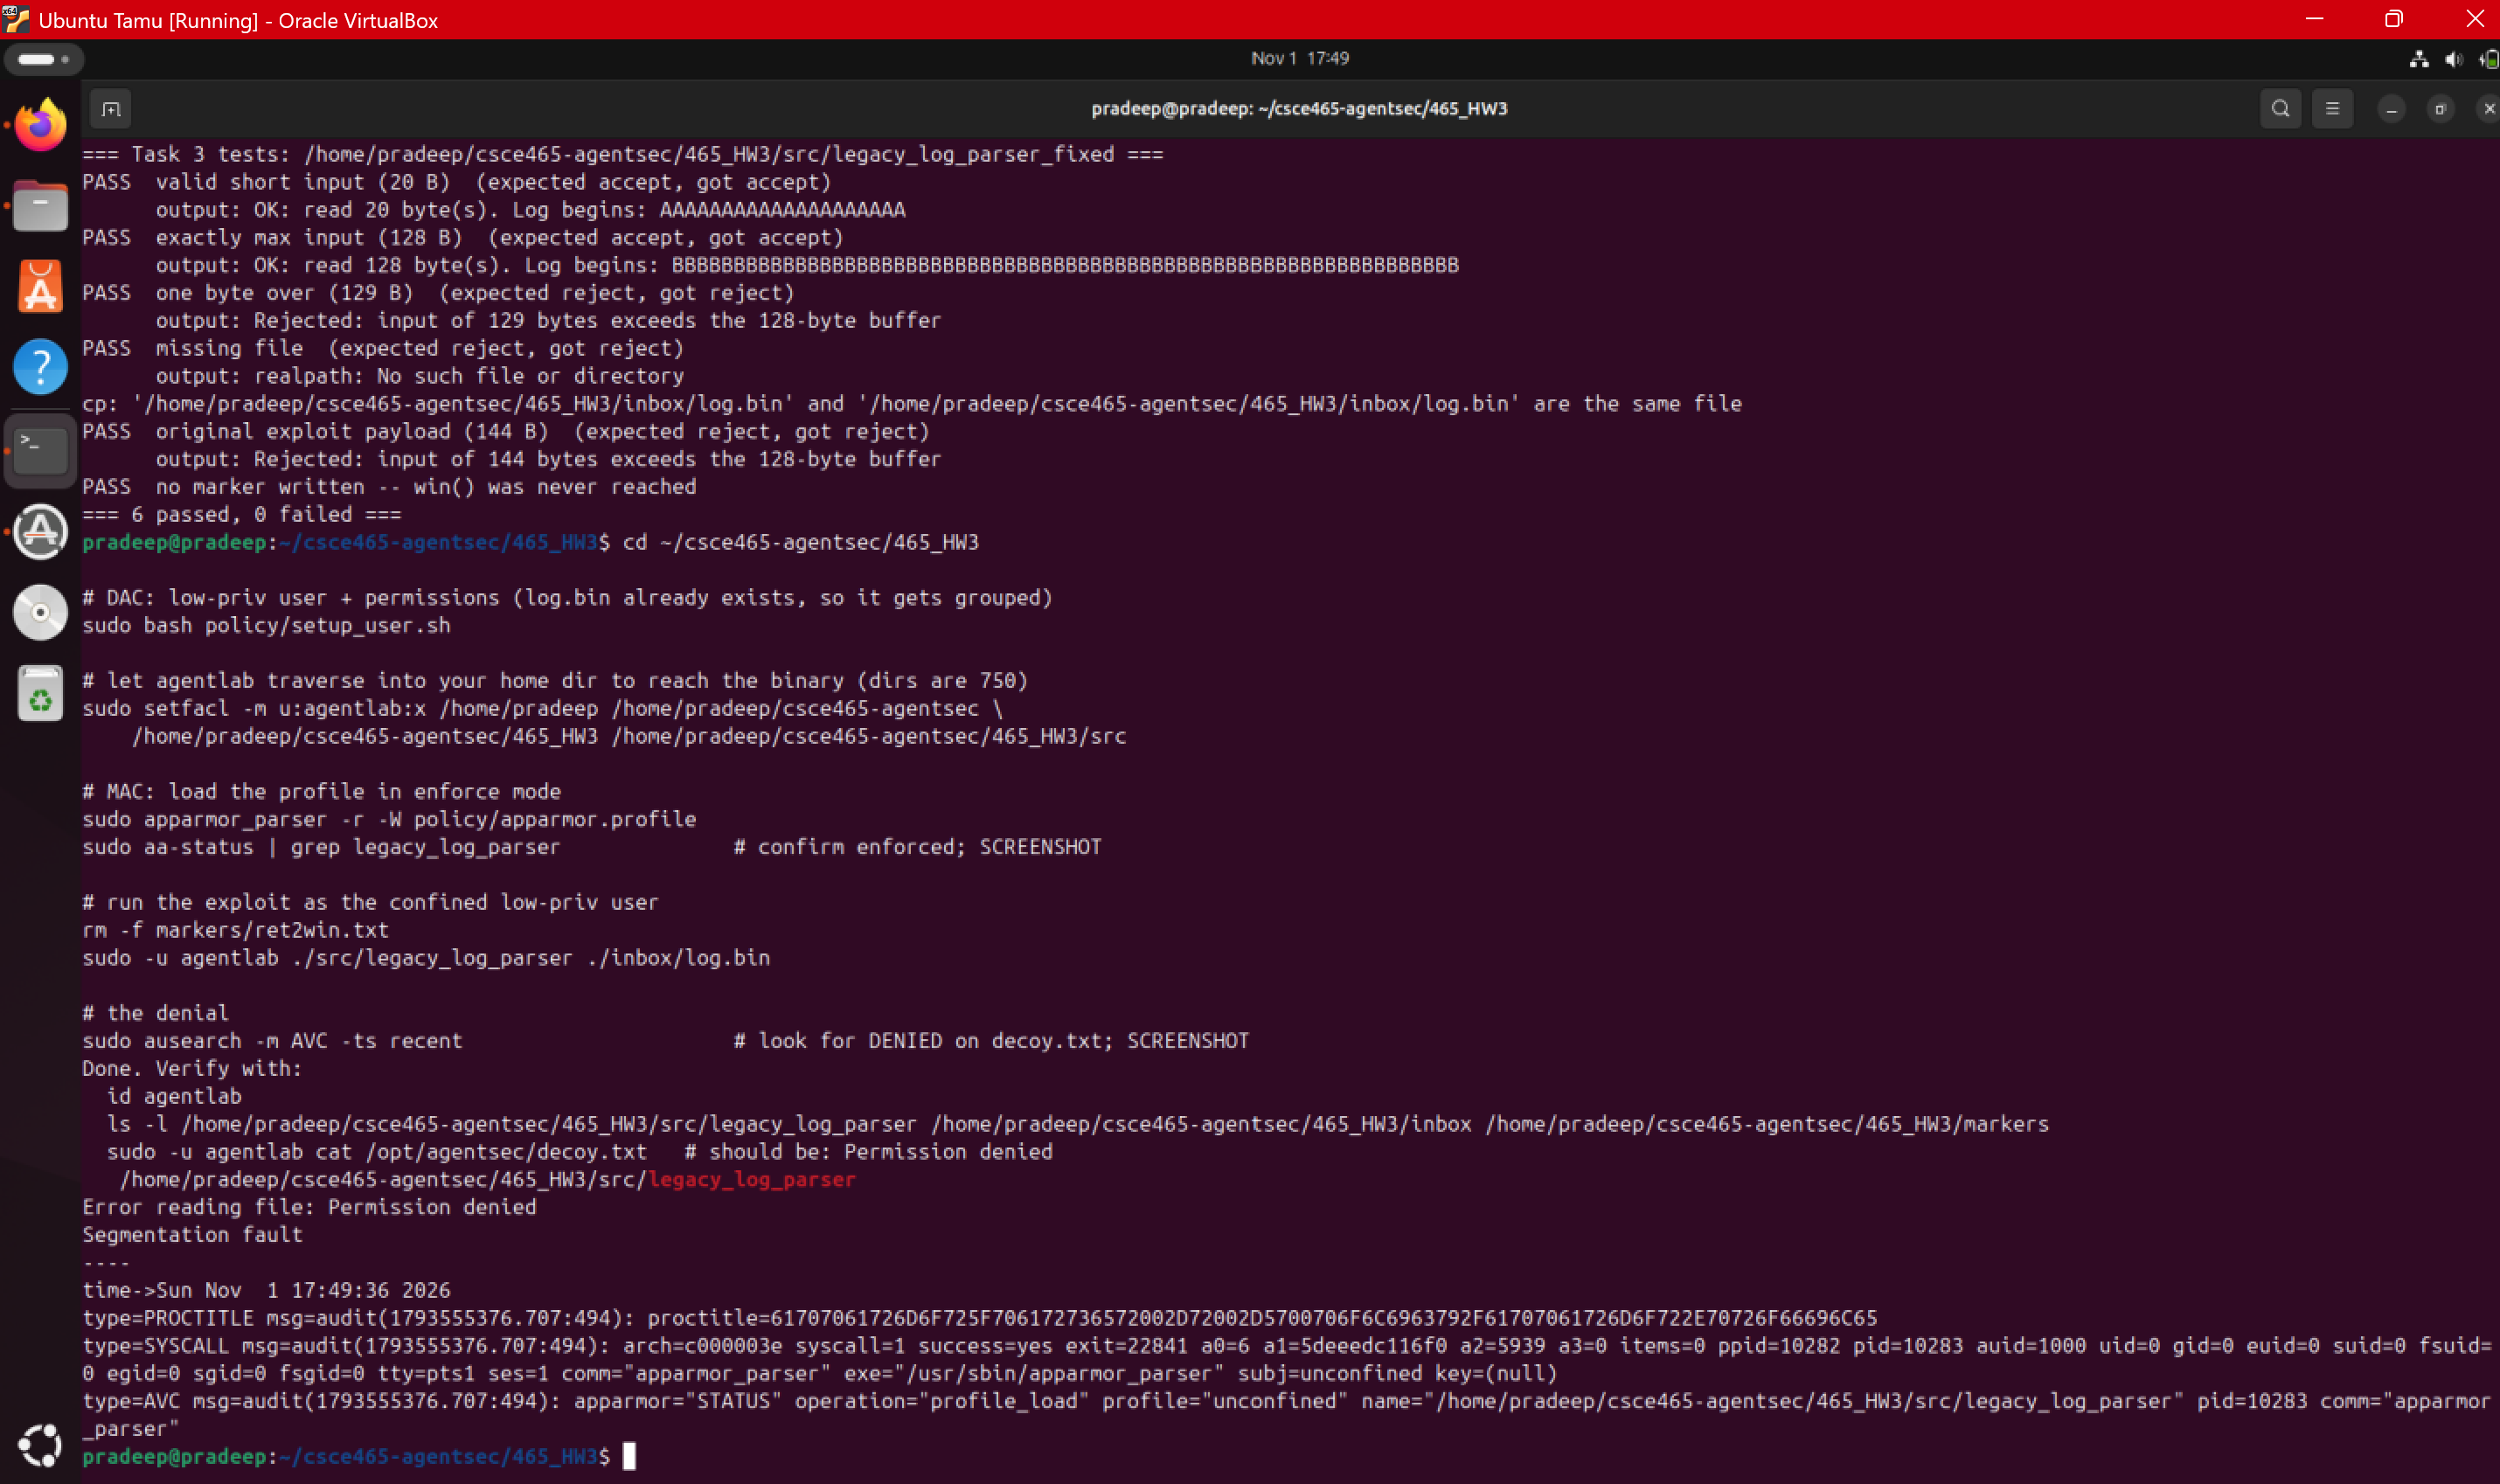
\includegraphics[width=\linewidth]{screenshots/04_task4_runA_agentlab.png}}
\caption{Run A (as \texttt{agentlab}): DAC blocks the decoy read; the only
AppArmor record is \texttt{STATUS}/\texttt{profile\_load}, i.e.\ no MAC denial is
needed because permissions already stopped the read.}
\end{figure}

\paragraph{Run B --- as root (MAC).}
Running as root means DAC would \emph{allow} the decoy read, isolating AppArmor.
The output shows ``Marker created'' followed by ``Cannot resolve entire path:
Permission denied,'' and the audit log records the denial:

\begin{lstlisting}
apparmor="DENIED" operation="capable" profile=".../legacy_log_parser"
    capname="dac_override"
apparmor="DENIED" operation="capable" profile=".../legacy_log_parser"
    capname="dac_read_search"
type=SYSCALL ... syscall=89 success=no exit=-13 ... subj=".../legacy_log_parser"
\end{lstlisting}

The \texttt{subj=} field confirms the process ran under the profile. Because the
profile grants no capabilities, AppArmor denied \texttt{dac\_override} /
\texttt{dac\_read\_search} --- the capabilities root would have needed to bypass
the decoy's permissions --- so the read failed with \texttt{exit=-13} (EACCES).
The marker was still written, so the exploit succeeded; MAC blocked only the
secret read. The denial surfaced as a \emph{capability} denial rather than a
file-open denial because, for an as-root access, the kernel first asks whether
the process may override DAC at all; the profile grants nothing, so it is
refused there. The explicit \texttt{audit deny} on the decoy is the
belt-and-suspenders that would catch the same access at the file layer for a
non-root run.

\begin{figure}[H]
\centering
\fbox{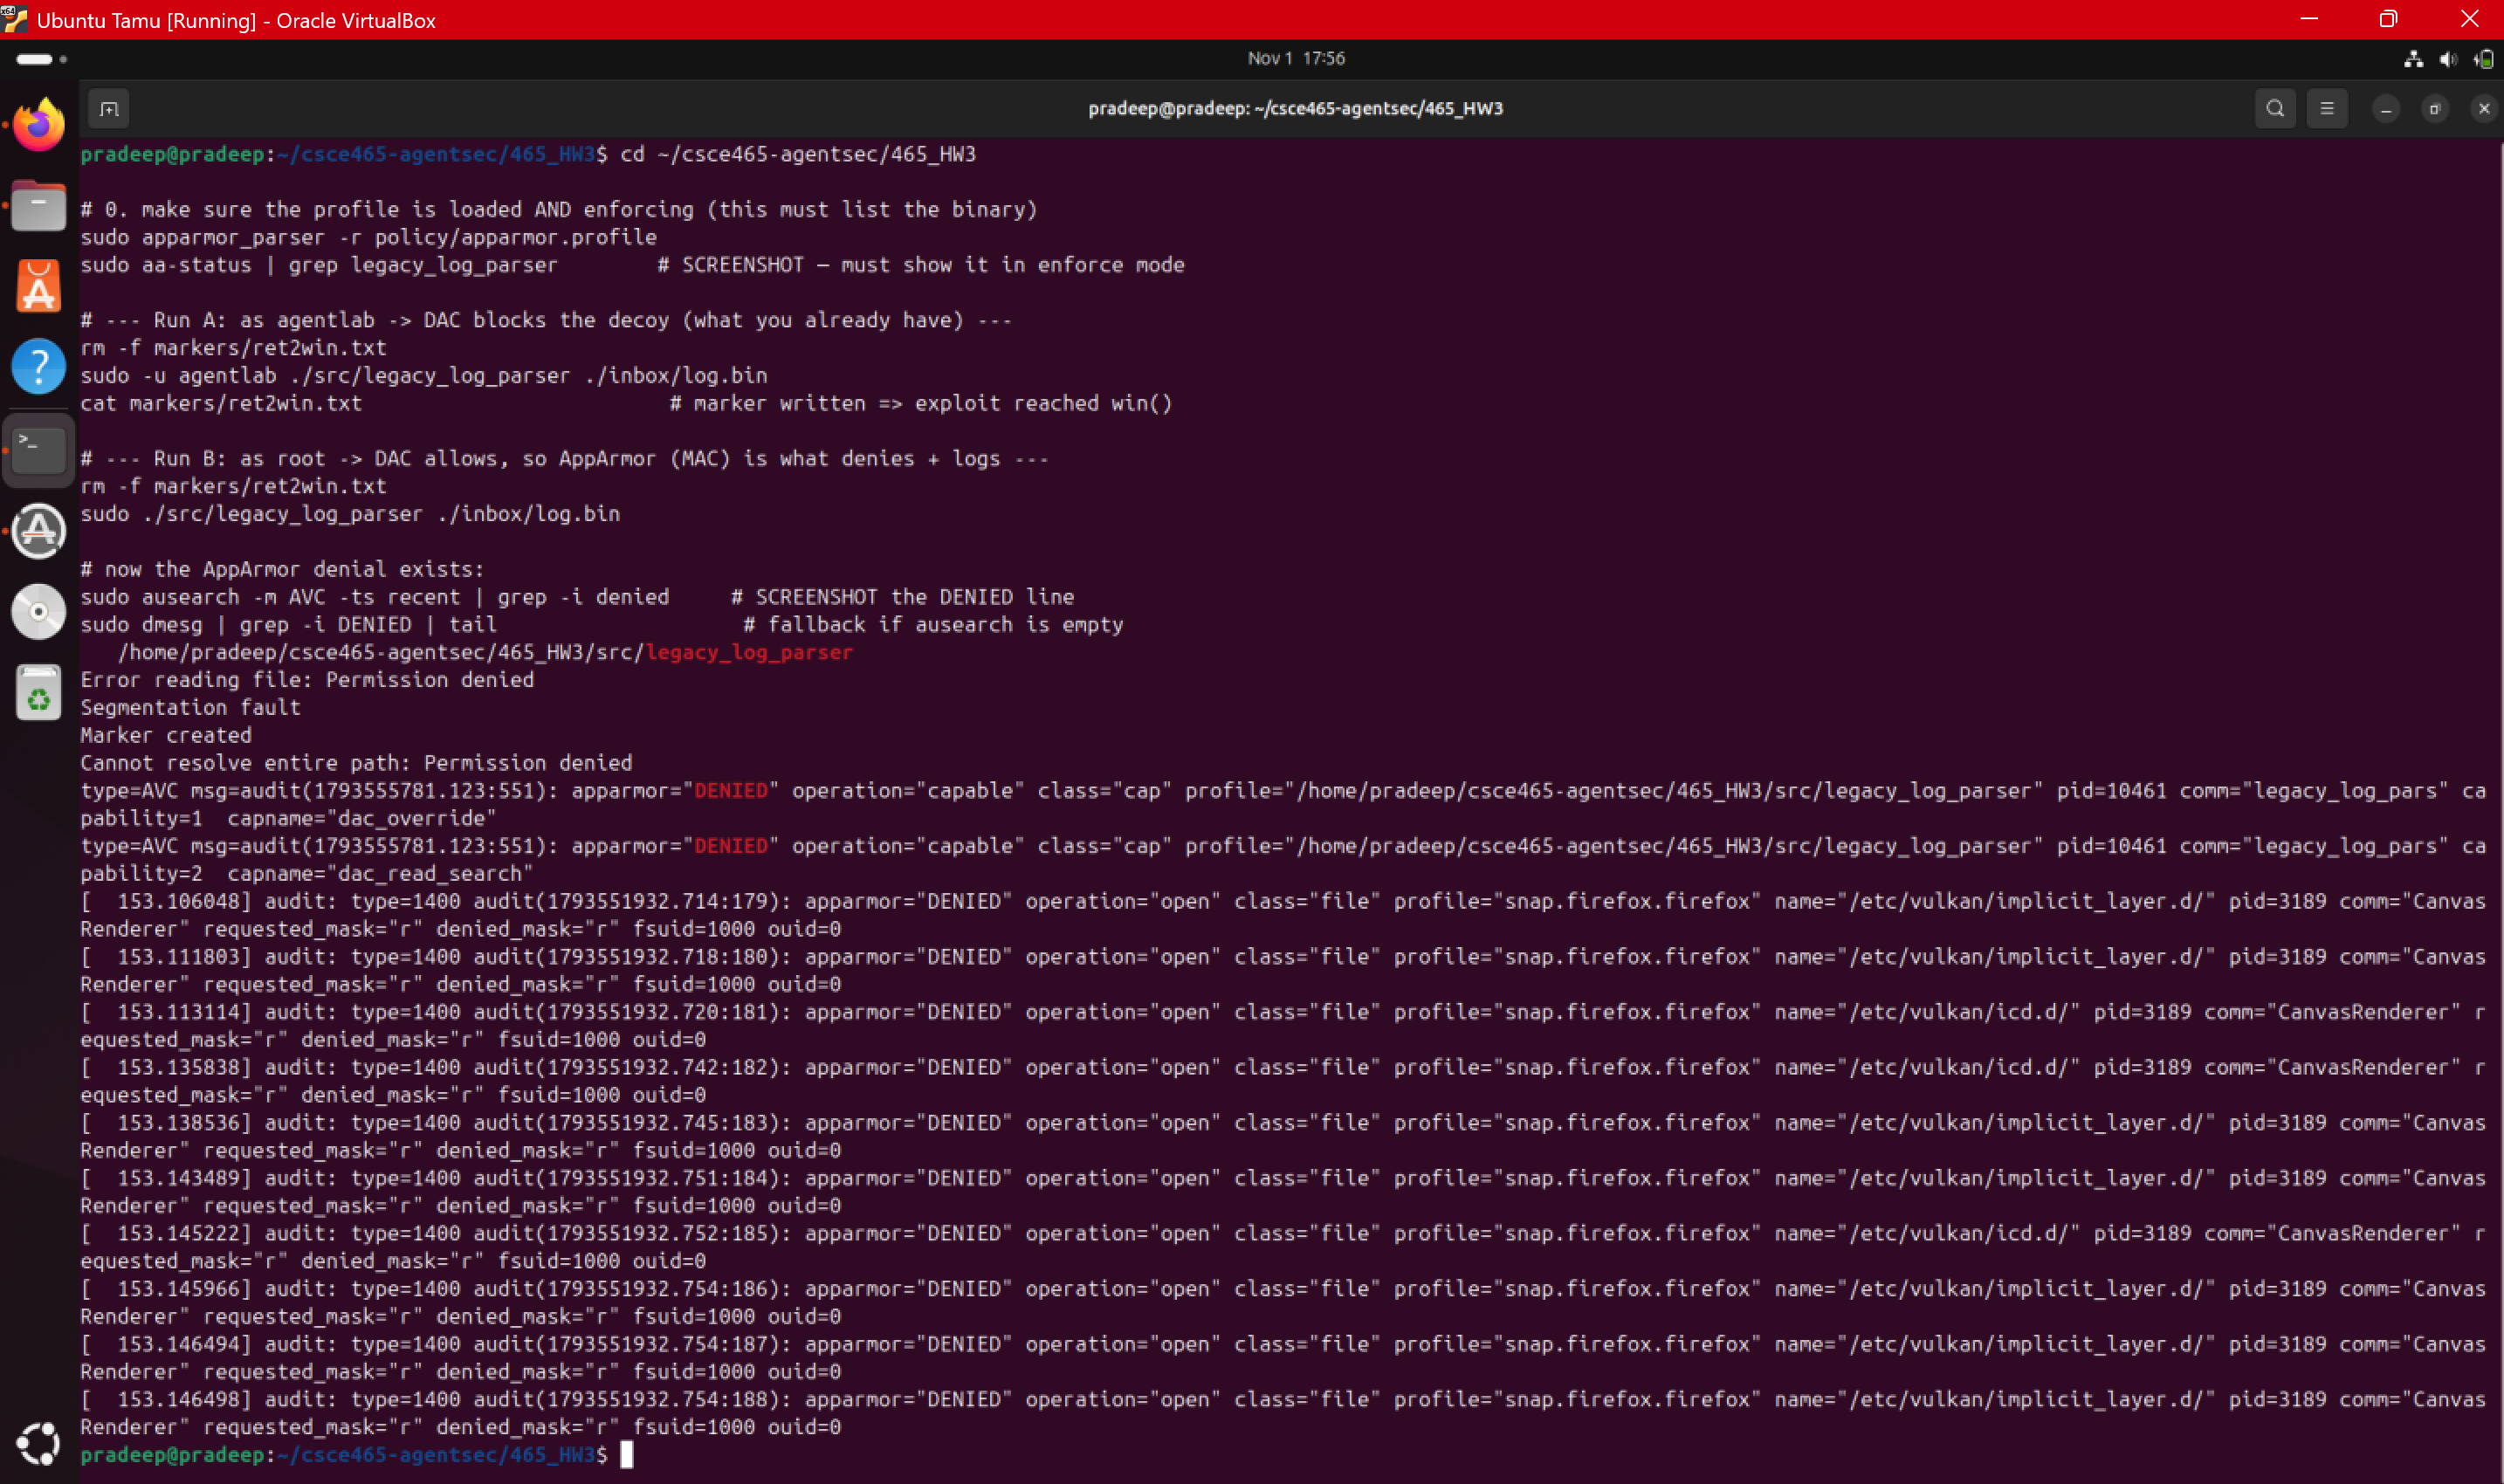
\includegraphics[width=\linewidth]{screenshots/05_task4_runB_denial.png}}
\caption{Run B (as root): the marker is created, then AppArmor denies the
\texttt{dac\_override} and \texttt{dac\_read\_search} capabilities, so the decoy
read fails with EACCES. The exploit succeeded; MAC contained it.}
\end{figure}

\begin{figure}[H]
\centering
\fbox{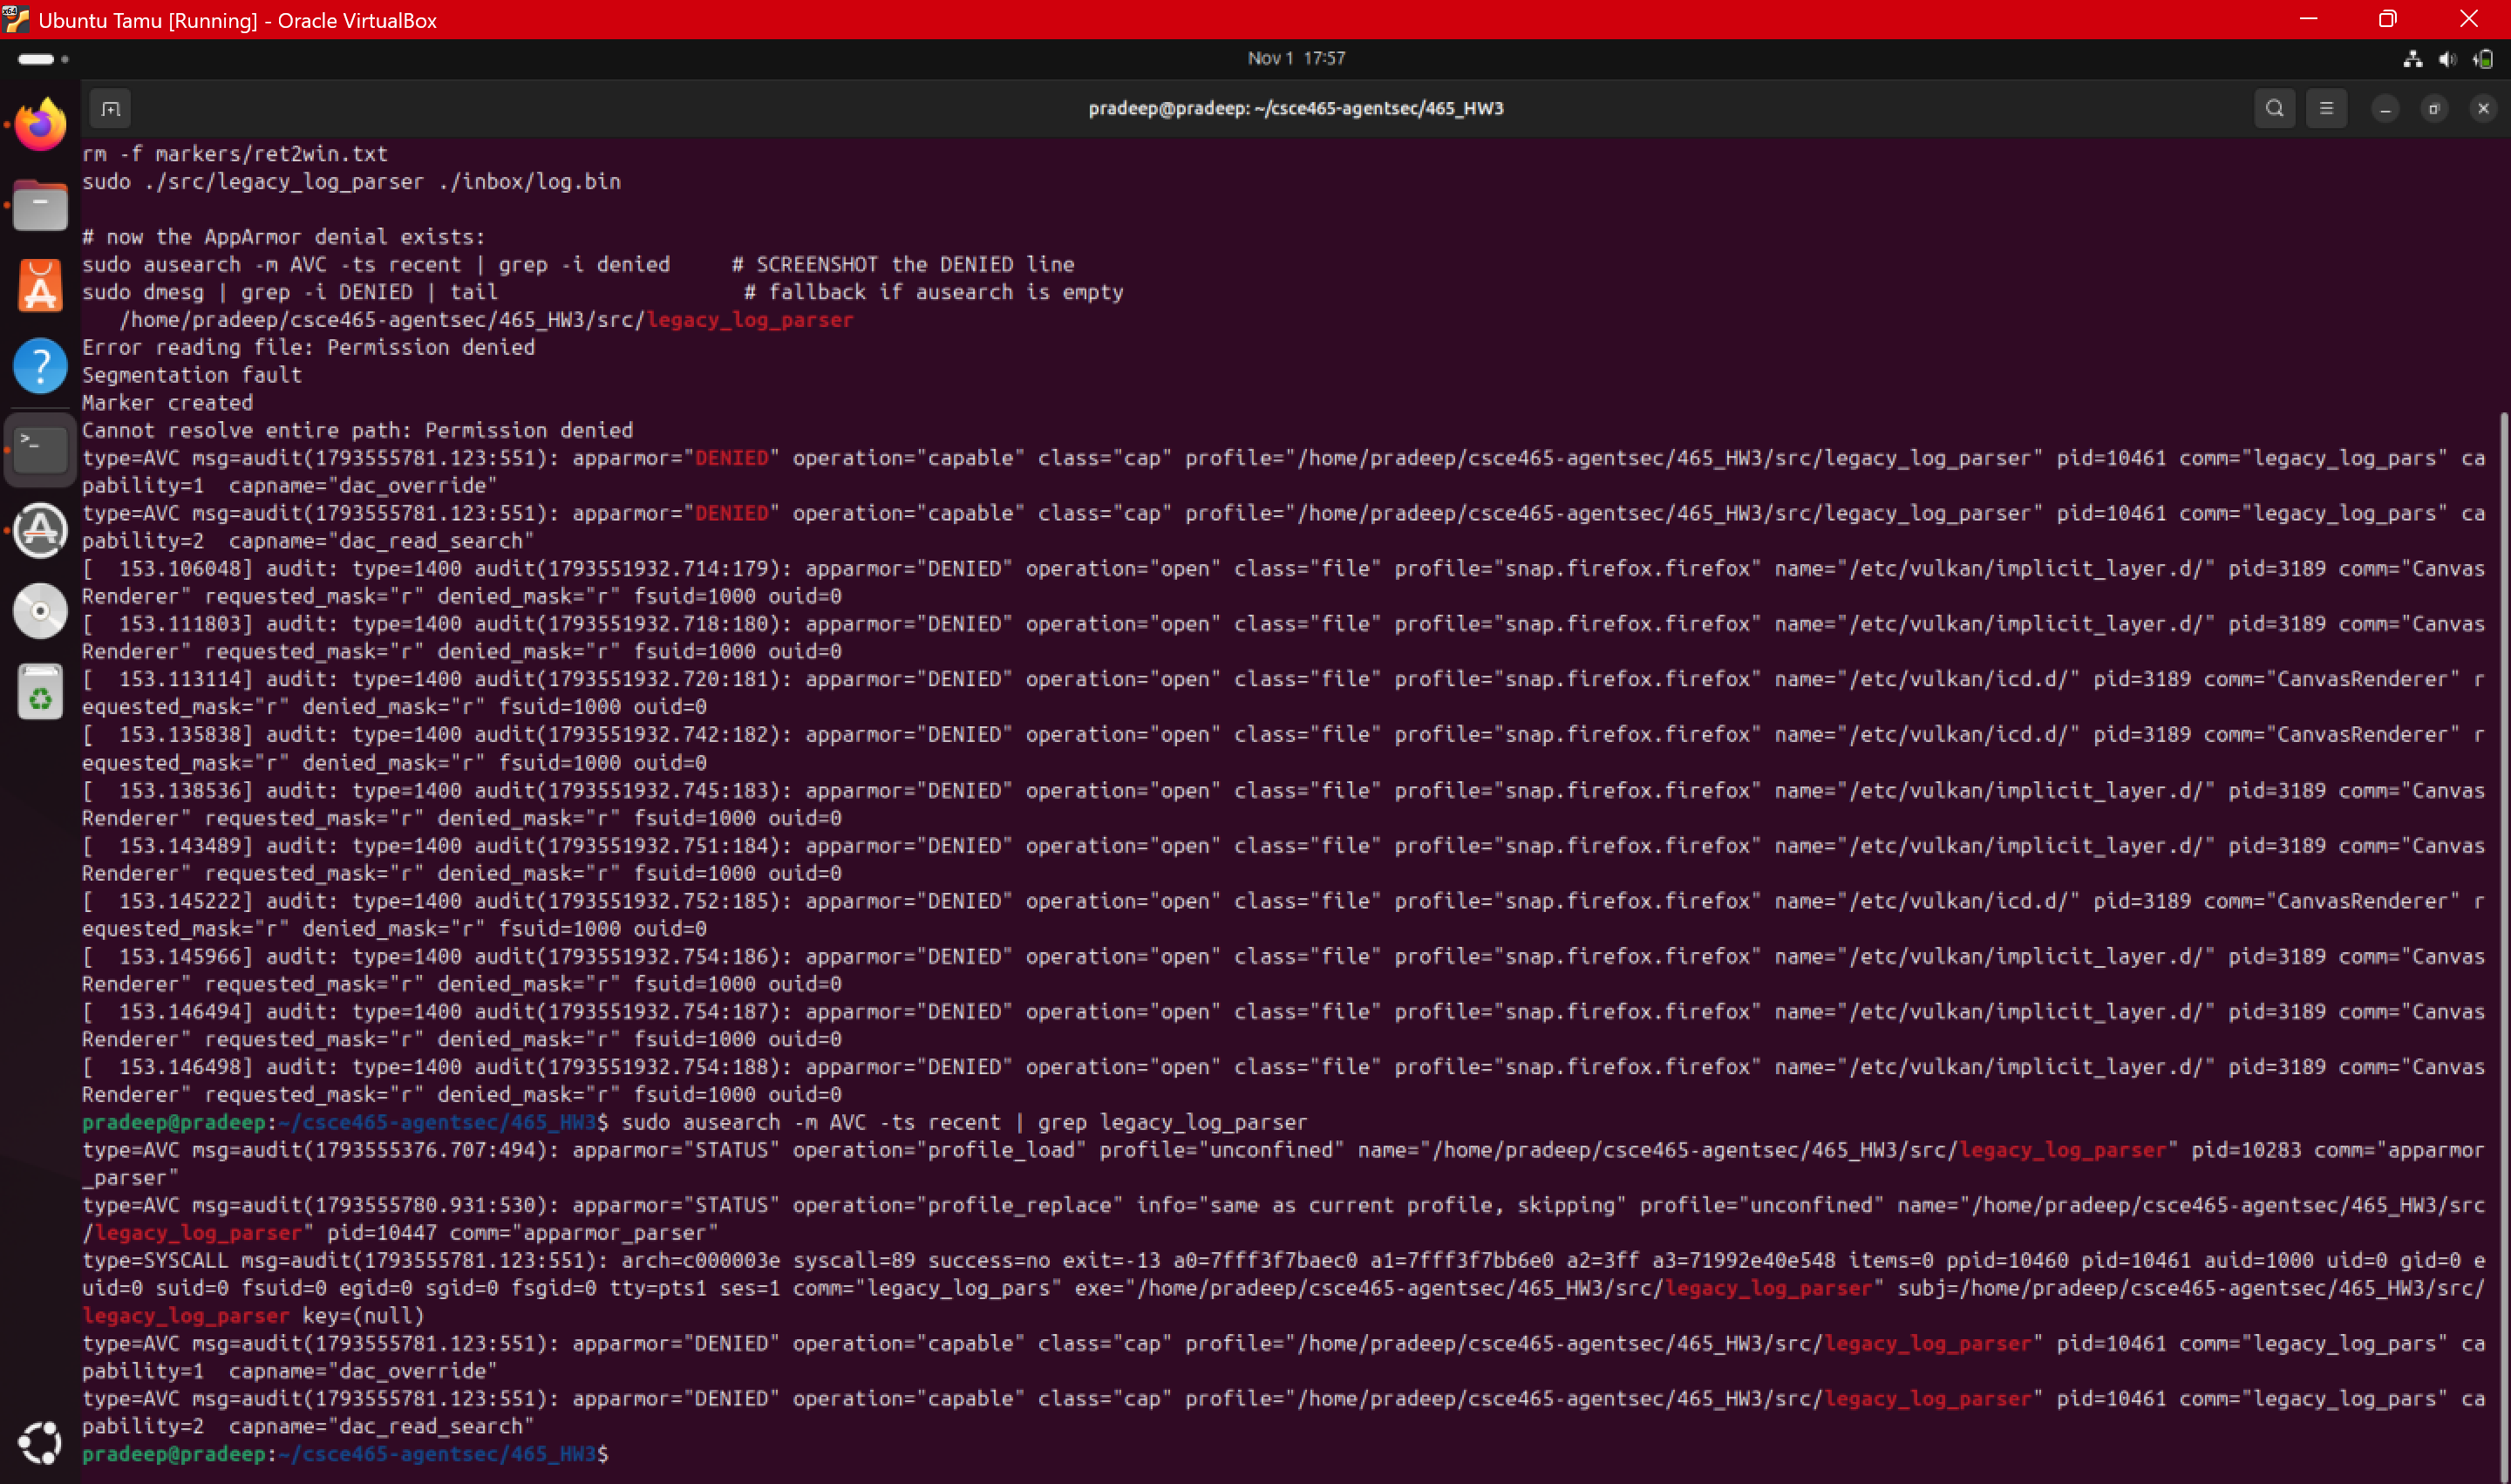
\includegraphics[width=\linewidth]{screenshots/06_task4_ausearch_filtered.png}}
\caption{\texttt{ausearch -m AVC -ts recent | grep legacy\_log\_parser} ---
filtered to the profile's own records: the \texttt{STATUS} loads, the failed
\texttt{SYSCALL} (\texttt{readlink}, \texttt{exit=-13}), and the two capability
\texttt{DENIED} lines.}
\end{figure}

\subsection{Reference monitor, complete mediation, access matrix, DAC, MAC, least privilege}
This experiment is a concrete instance of the Chapter~5 access-control model. A
\textbf{reference monitor} is the component between every subject and every
object that checks each access against a policy; to be trustworthy it must be
tamper-proof, always invoked, and small enough to verify. Here the kernel's
AppArmor LSM is the reference monitor for the parser: every \texttt{open},
\texttt{read}, \texttt{write}, and capability request the confined process makes
is intercepted in kernel space, which the process cannot bypass.

\textbf{Complete mediation} is the requirement that no access escapes that
check. The experiment relies on it directly: the exploit does not use the
parser's intended interface --- it corrupts the return address to jump into
\texttt{win()}. Because mediation is complete, it does not matter \emph{how}
execution arrived at the decoy access; the kernel still mediates it (Run B's
capability check) and denies it. A monitor that only checked the ``intended''
code path would be defeated by exactly this control-flow hijack.

The \textbf{access matrix} is the conceptual table of which subjects may do what
to which objects. The two layers fill it from two directions. The row for
subject \texttt{agentlab} is set by \textbf{DAC} --- the ownership and
permission bits in \file{setup\_user.sh} (\texttt{750} binary, \texttt{640}
inbox files, \texttt{770} markers, \texttt{600} root-only decoy). DAC is
\emph{discretionary} because the file owner sets these and can change or
delegate them; its weakness is that a program a user runs inherits that user's
full rights.

\textbf{MAC} fills the column for the \emph{program}. The AppArmor profile is a
system-level policy bound to the binary that the invoking user cannot override
--- not even root running the program. This is why both layers matter: in Run A,
DAC stops the unprivileged \texttt{agentlab}; in Run B, MAC stops the
\emph{process itself} even when it runs as root and DAC would have allowed the
read. Each enforces the same restriction independently --- neither alone is
sufficient, and together they survive a failure of the C code.

\textbf{Least privilege} ties it together: every grant is the minimum needed.
The DAC user can touch exactly three paths; the MAC profile allows read of
\file{inbox/}, write of \file{markers/}, the loader and libc, and nothing else
--- no shell execution and no capabilities. The ret2win attack is not
\emph{repaired} by any of this; the overflow is still present, and the marker is
still written in both runs. What confinement changes is the blast radius: a
defect that would otherwise read a protected secret (and could pivot to a shell)
is reduced to writing one marker file in one directory, because the reference
monitor completely mediates each access and the policy grants almost nothing.
That is the assignment's thesis --- attack (Task 1), mitigate (Task 3), contain
(Task 4) --- with no single layer trusted to be enough.

\section*{Reproducibility}
\addcontentsline{toc}{section}{Reproducibility}
Full build/run/confine commands are in \file{README.md}. In brief, from
\file{\textasciitilde/csce465-agentsec/465\_HW3}: build both binaries, run
\file{tests/run\_tests.sh} (Task~3), then \file{sudo bash policy/setup\_user.sh}
and \texttt{sudo apparmor\_parser -r -W policy/apparmor.profile}, and capture
the denial with \texttt{sudo ausearch -m AVC -ts recent}. Paths assume the user
\texttt{pradeep}; adjust \texttt{INBOX\_DIR} and the profile paths otherwise.

\end{document}
